\chapter{Összegzés}
\section{Az elért eredmény}
Az alkalmazás beüzemelése sikerült, és büszke vagyok arra a megoldásra amit építettem. Három privát GitHub repositoryban található a három alkalmazáskomponens, mindegyiken külön dedikált \textit{prod} (az éles, felhasználók számára látható verzió), és \textit{beta} (fejlesztők számára, az élessel megegyező környezetben futó tesztverzió) ág. Mindkét ág \textit{branch protection}nel van ellátva, arra leadott pull request csak akkor fogadható el ha annak Jenkins buildje sikeresen lefutott.

CI/CD szempontjából sikerült elérni a várakozásokat. A GitHubbal koordináltan zajlik a kiemelt ágak és pull requestek ellenőrzése (más ágaké nem, a buildszerver indokolatlan leterheltségének megelőzése érdekében). Amennyiben a Jenkins sikeresen lebuildeli az alkalmazást, akkor a konténerképet privát ECR repositoryba küldi és alkalmazza a Kubernetesben a változtatásokat, lépcsőzetes frissítés segítségével. Ha valami a tesztek ellenére balul sülne el, akkor a deployment manuális szerkesztésével, a konténerkép verziószámának (ami a \textit{tag}je) átírásával gyorsan vissza lehet állni korábbi verzióra.
\begin{figure}[ht]
\centering
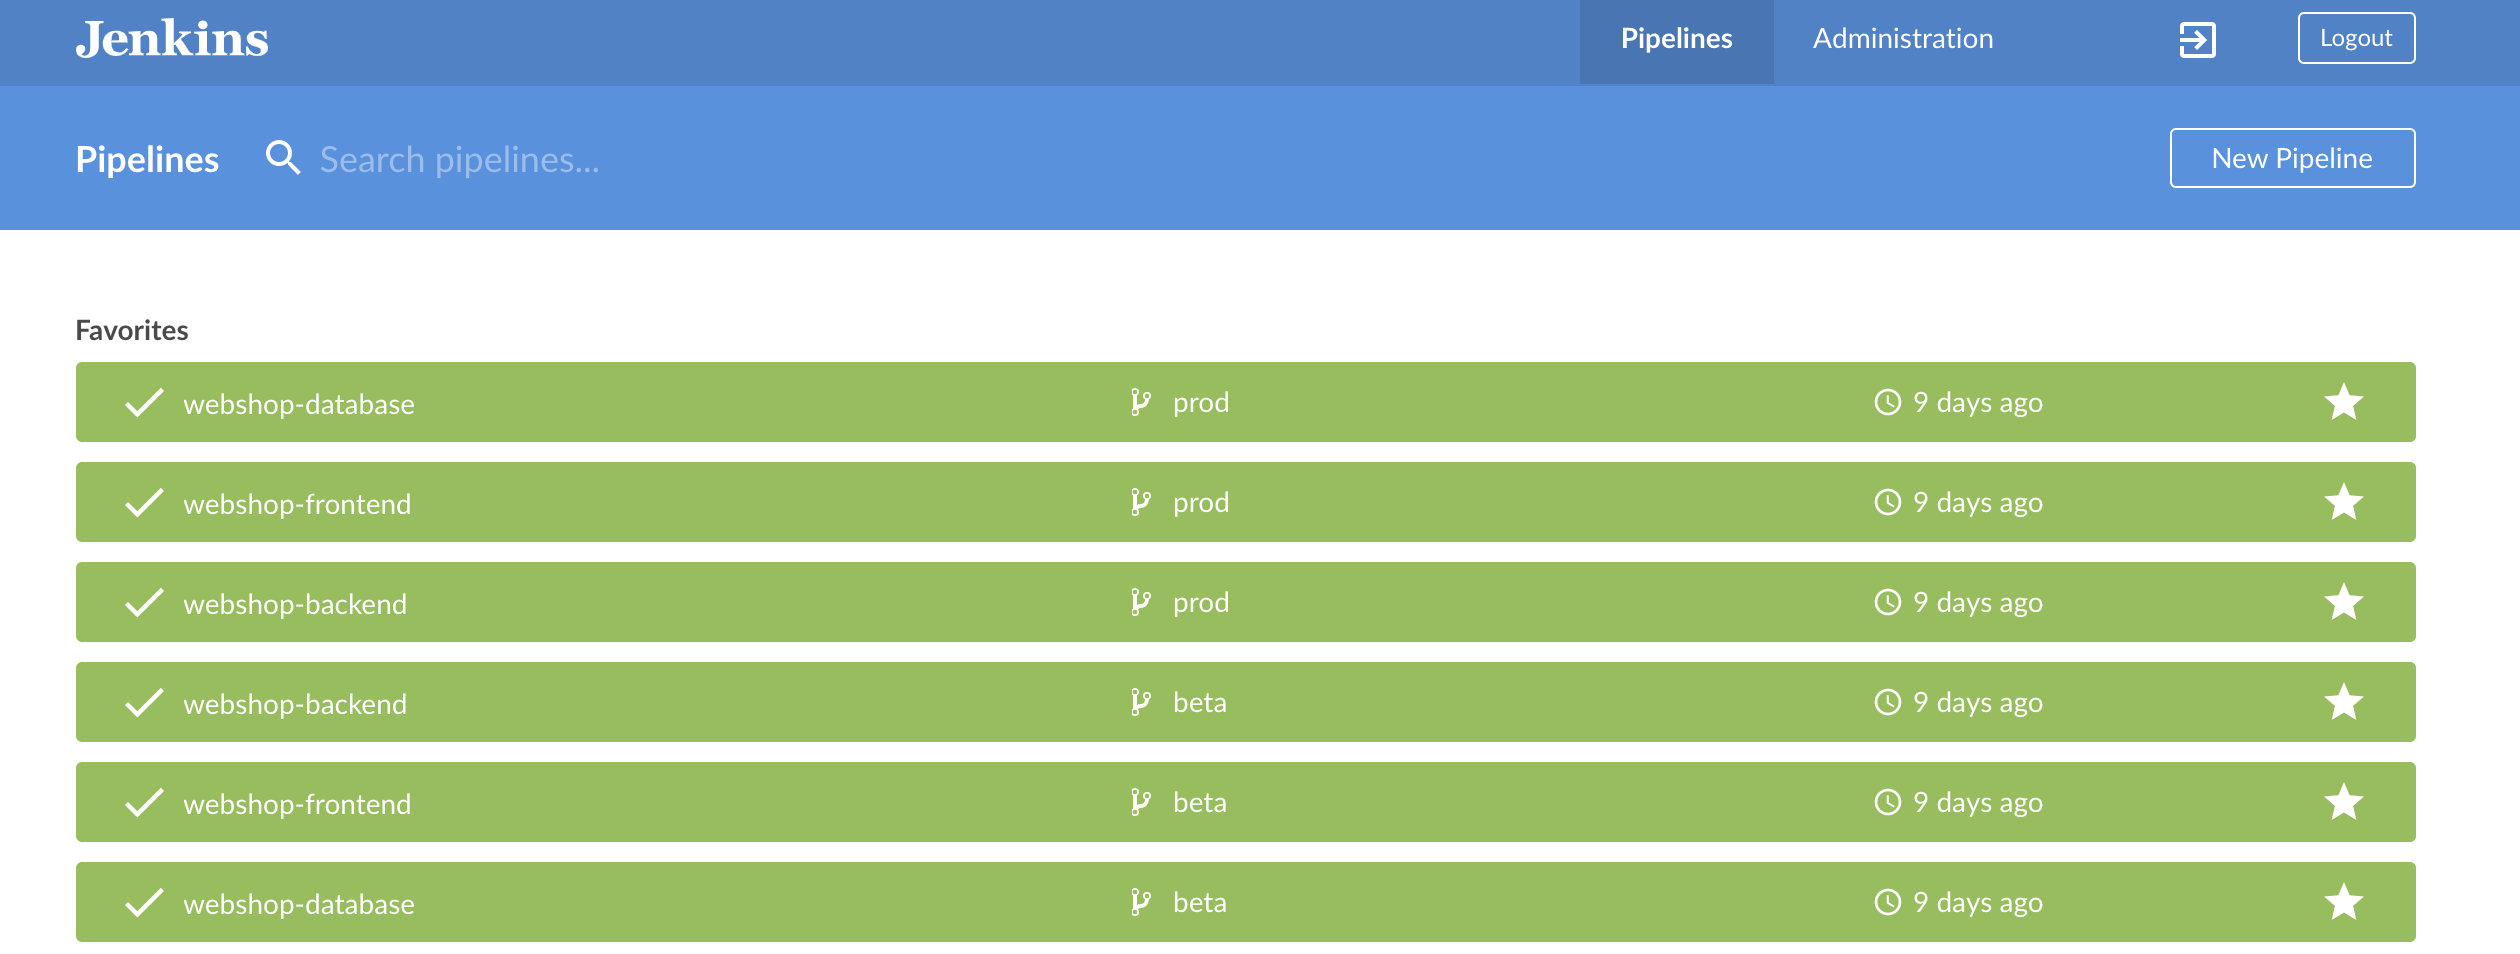
\includegraphics[width=150mm, keepaspectratio]{img/jenkinsgreen.png}
\caption{Minden ág sikeresen lefordul és települ}
\end{figure}
\vskip 0.1in
Az alkalmazás automatikusan skálázódik, mégpedig minden komponense. Egységesen 50\% CPU használatra van beállítva mindhárom rész. Az adatbázis az állapotfüggőségből adódóan nem skálázható teljesen: a Postgres úgynevezett \textit{master-slave replikáció}t használ, ami azt jelenti, hogy bár egyszerre több példányt is lehet olvasni, írni csak és kizárólag a mesterpéldányt lehet. A gyakorlatban tehát az adatbázisnak csak az olvasási teljesítménye skálázható, az írási kizárólag vertikálisan (azaz több erőforrás hozzáadásával) növelhető.
\clearpage
\begin{figure}[!ht]
\centering
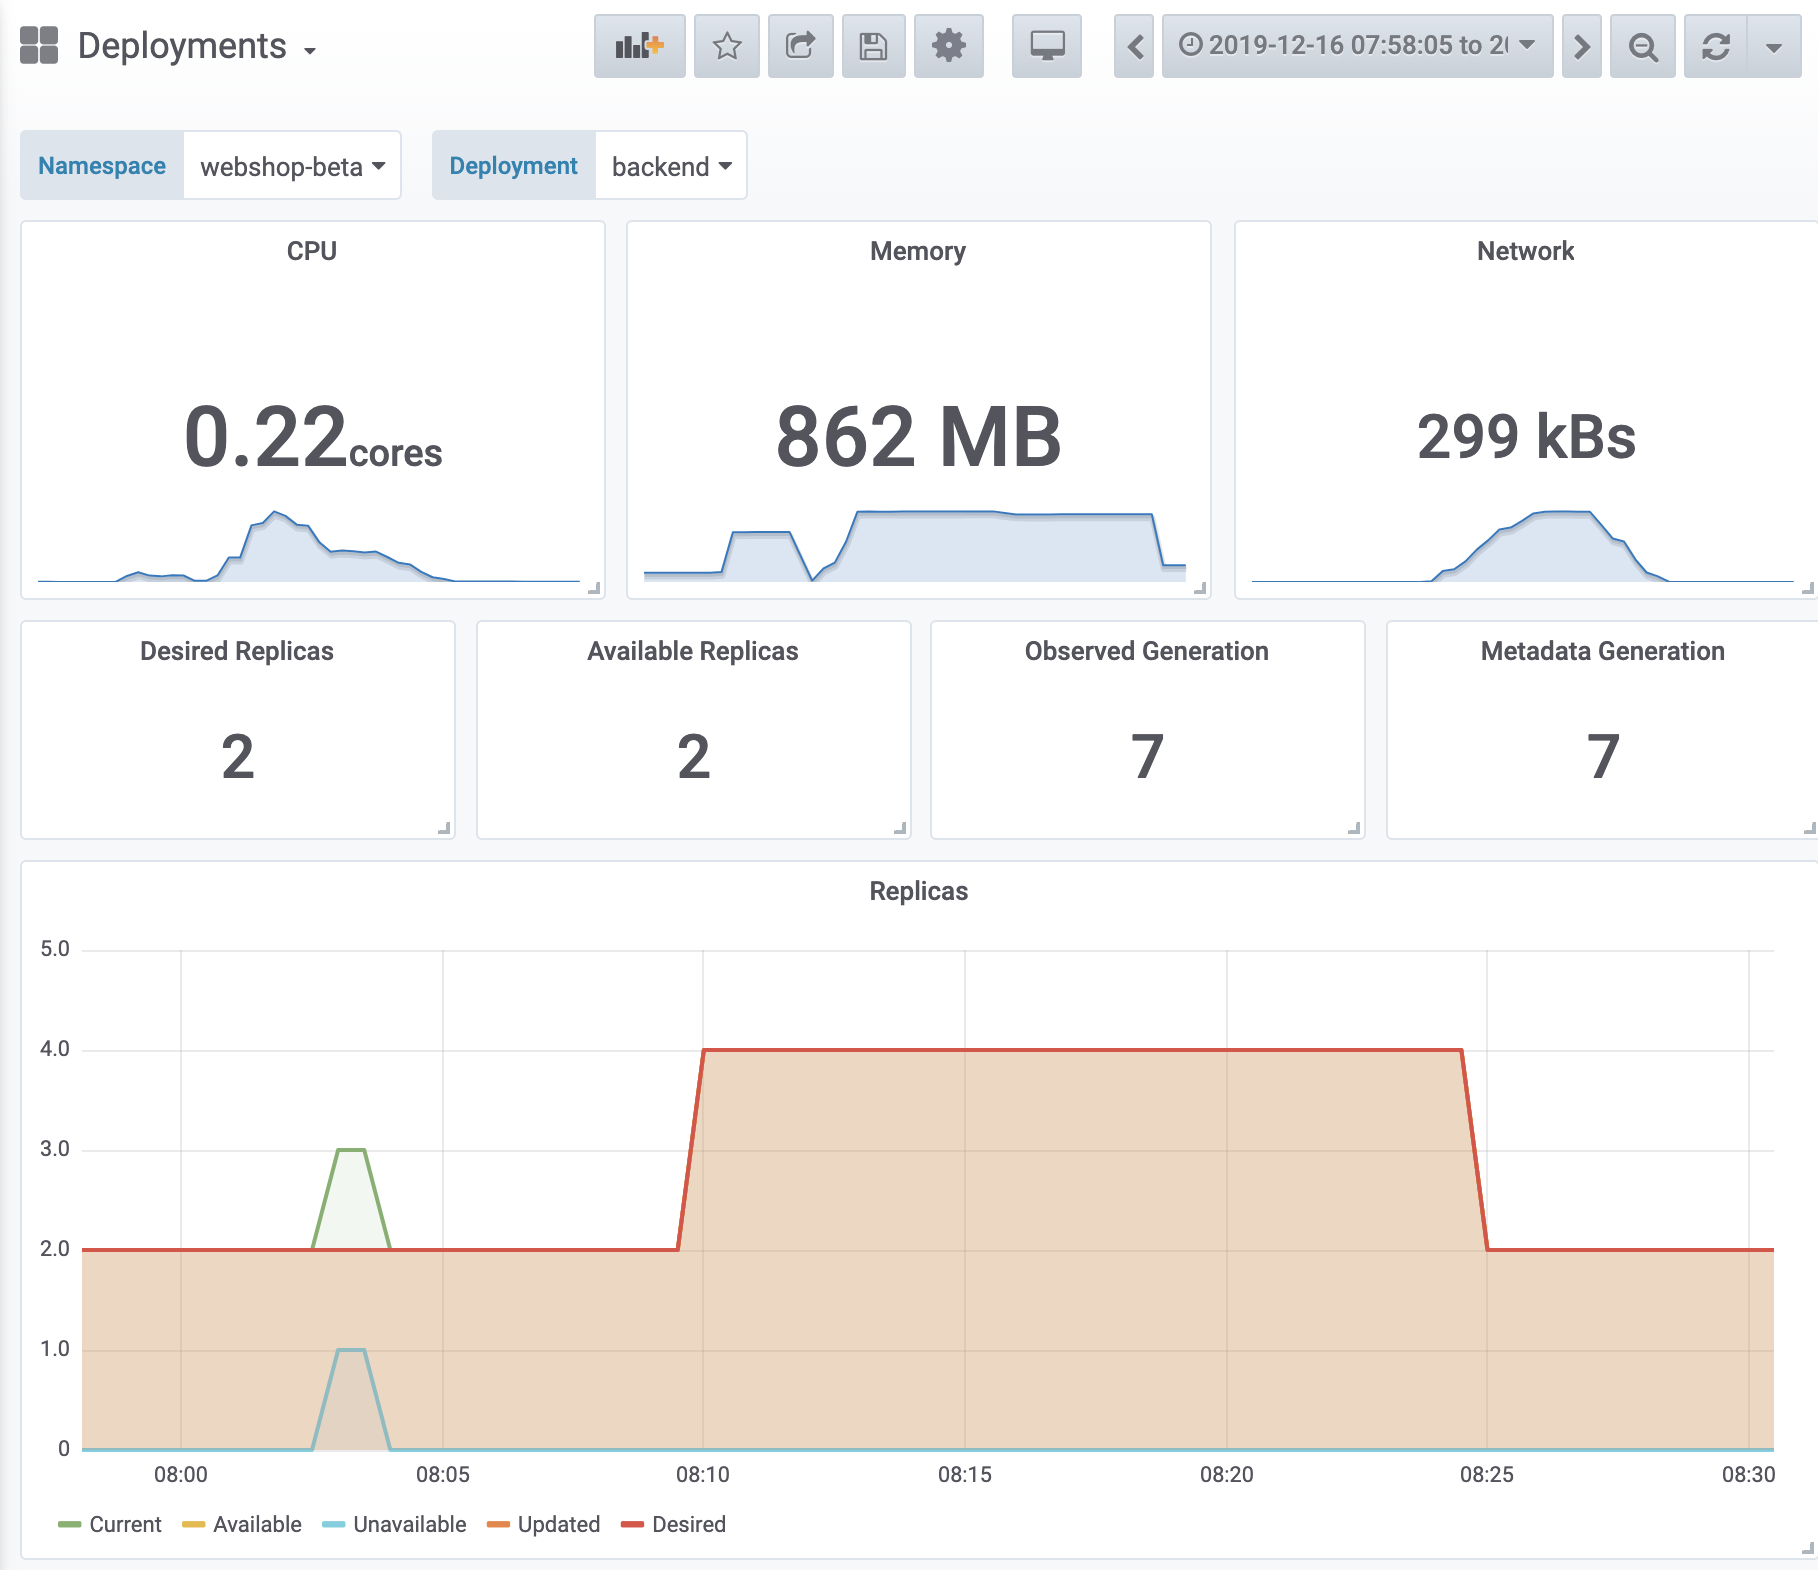
\includegraphics[width=150mm, keepaspectratio]{img/replica_up.png}
\vskip 0.5in
\vfill
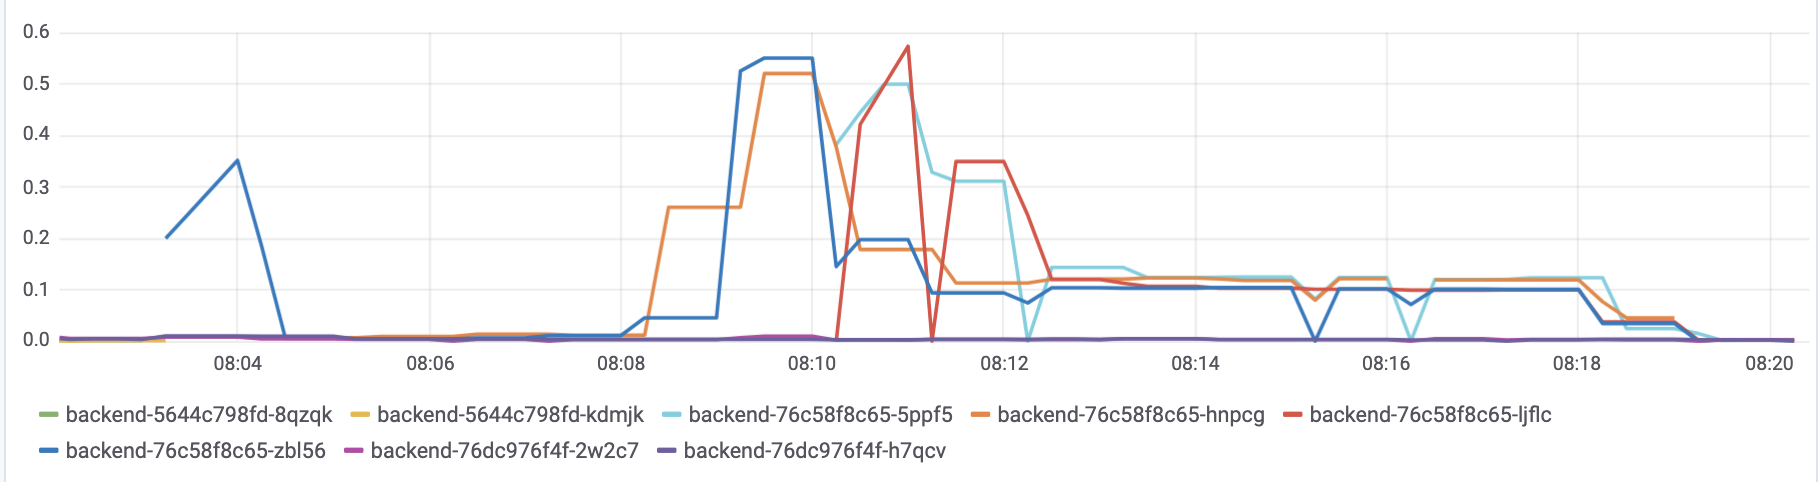
\includegraphics[width=150mm, keepaspectratio]{img/hpa_cpu.png}
\caption{Terhelés hatására új példányok indulnak, a processzorhasználat normalizálódik}
\end{figure}
\clearpage
Monitorozás szempontjából minden részkomponens a Kubernetes adta readiness és liveness ellenőrzésekkel el van látva (HTTP státuszkód 200 (OK) kell legyen a visszatérési státuszkód), ha meghibásodik valamelyik akkor az automatikusan törlésre kerül és új példány indul belőle. A magas rendelkezésreállás is garantált mivel minden komponens minimum két példányban fut. Ez az adatbázisra is igaz, ugyanis a mester halála esetén az alárendelt példány ideiglenesen átveszi a mester feladatát, írhatóvá válik, majd a mester újraéledése során visszaszinkronizálja az adatokat és minden visszaáll eredeti állapotába.
\section{Nehézségek}
Az első komoly kihívást előre sejtettem: állapotfüggő alkalmazást szerettem volna több példány indításával skálázni, az adatbázist. Ez egy meglehetősen bonyolult feladatnak bizonyult, ráadásul az eredetileg az alkalmazás által használt \textit{HyperSQL}-t nem ismertem. Kutatásom során rájöttem, hogy csak replikációt támogató adatbázissal megoldható a probléma, és azzal sem feltétlenül egyszerűen. Egy útmutató példa volt a népszerű MySQL Kubernetesbe helyezéséről szóló dokumentáció\cite{db_k8s}, és kis olvasás után rájöttem, hogy a számomra jobban ismert Postgres is skálázhatóvá tehető, ha csak olvasási teljesítményben is.

Egy másik probléma a Jenkins pipeline kialakításakor került elő: \textit{Multistage Dockerfile}ok segítségével fordítottam a projekteket, ami gyakorlati szempontból annyit jelent, hogy egy Docker motor elérhető kell legyen a Jenkins számára. Mivel én már magát a Jenkinst is Kubernetesben futtattam (ami pedig Dockerre épít), így egy érdekes megoldást választottam (és fenntartom, hogy nem ez a legoptimálisabb megoldás): Docker in Docker konténert is definiáltam a Jenkinshez tartozó Podba (\textit{emlékeztető: A Pod a Kubernetes legkisebb egysége, konténerek összessége}) majd a Jenkinsen átadtam a megfelelő \lstinline{DOCKER_HOST} környezeti változót, illetve egy egyedi Jenkins konténerképet csináltam, melybe többek között egy Docker klienst is elhelyeztem.

Hasonló problémába ütköztem a Kubernetesbe való alkalmazástelepítéskor is. Nem tudtam könnyedén kommunikálni a Kubernetes API-val ugyanis hiányzott a \textit{kubectl} nevű eszköz mely ezt a feladatot látja el. Szintén az egyedi konténerképben helyeztem el, ami elérhető DockerHubon\footnote{\url{https://hub.docker.com/repository/docker/msbence/jenkins-docker-kubectl} \newline msbence/jenkins-docker-kubectl:aws}. Az ehhez tartozó Dockerfile itt található:
\begin{lstlisting}
FROM jenkins/jenkins:lts
USER root
RUN apt-get update && \
apt-get -y install apt-transport-https \
     ca-certificates curl gnupg2 python3-pip \
     gettext \
     software-properties-common && \
curl -fsSL https://download.docker.com/linux/$(. /etc/os-release; echo "$ID")/gpg > /tmp/dkey; apt-key add /tmp/dkey && \
add-apt-repository \
   "deb [arch=amd64] https://download.docker.com/linux/$(. /etc/os-release; echo "$ID") \
   $(lsb_release -cs) \
   stable" && \
apt-get update && \
apt-get -y install docker-ce
RUN apt-get install -y docker-ce
RUN usermod -a -G docker jenkins
RUN curl -LO https://storage.googleapis.com/kubernetes-release/release/$(curl -s https://storage.googleapis.com/kubernetes-release/release/stable.txt)/bin/linux/amd64/kubectl \
    && chmod +x ./kubectl \
    && mv ./kubectl /usr/local/bin/kubectl
RUN pip3 install awscli --upgrade
USER jenkins
\end{lstlisting}

Az utolsó két problémám abból eredt, hogy az infrastruktúrát egy külsős cég finanszírozta és az Ő Amazon fiókjuk alá kaptam egy alfiókot. Értelemszerűen nem kaphattam mindenhez hozzáférést, illetve nem láthatam bele a rendszereikbe. A korlátozásokat sok módon próbáltuk a konzulesemmel együtt bevezetni, de végül a megoldás egy külön AWS régióra korlátozás lett. Ettől függetlenül sokszor kellett még apróbb engedélyeket kérnem, ráadásul az AWS IAM nem egy egyszerűen kiismerhető rendszer. Ebből adódóan sokszor hanyag voltam a jogosultságkezelés terén, mert több IAM szerepet kell volna létrehozni, mint amennyit én használtam. Ez viszont rengeteg többletidőt igényelt volna. Ahol szuboptimális megoldást válaszotottam ott ezt jeleztem is. A másik probléma, hogy az \textit{Elastic Kubernetes Service} drága mivolta miatt nem jutottam hozzá hamar a fiókhoz, ezért Google Cloud Platformon kezdtem el megcsinálni a dolgozatom. Egy ideig ez megoldásnak bizonyult és sokat segített, azonban az idő előrehaladtával egyre több Google-specifikus konfiguráció jött elő, és nem tudtam mindent követni, továbbá a hivatkozott forrásaim is mind a Google rendszeréhez kapcsolódtak volna. Végül időben kaptam hozzáférést, de tanulságos volt, hogy milyen különbség van két felhőszolgáltató között, még akkor is, ha ugyanazt a szolgáltatást nyújtják.
\section{Továbbfejlesztési lehetőségek}
Bár büszke vagyok a megoldásomra, azt gondolom hogy azt még lehet fejleszteni, hogy a gyakorlati használatra jobban fel legyen készítve. Az egyik ilyen a már fentebb említett IAM részletesebb kidolgozása. Például célravezetőbb lenne külön egy IAM role a Jenkins számára és nem a klaszterét használni. Ez biztonsági megfontolásokból előnyös leginkább. Azonban mivel az alapértelemezett szerep amit a podok látnak az a worker node IAM role, és ezt sikeresen átállítottam, így a podonkénti jogosultságkezelést demostrálni tudtam.
Egy másik pont ahol lehetne fejleszteni a rendszeren az a deploymentek kezelése, azaz az alkamazás kiadásának folyamata. Jelenleg az egyetlen verziókezelési (és ezzel visszaállítási) mód a konténerképek címkéi, ami a Jenkins buildszám. Például a Helm\footnote{Kubernetes csomagkezelő} bevezetésével ez a folyamat egyszerűbb és vizualizálhatóbb lenne. Ami viszont igazán pratikus lenne az egy külön deployment felület: jelenleg a \textit{prod} ágra helyezett programkód automatikusan kerül ki a felhasználók elé. Ezt át lehetne helyezni mondjuk egy weboldalra, ahol kézzel lehet az alkalmazást frissíteni, amennyiben azt a Jenkins sikeresen lefordította (és tesztelte), illetve könnyen lehet verziót visszavonni is.
A harmadik pont nem tartozik a szakdolgozatomhoz semmilyen mértékben, azonban a probléma fontossága miatt egy mondatban megemlítem: a példaalkalmazáshoz teszteket lenne szükéges írni, hiszen a \textit{Continuous Integration}nak ez az egyik lényeges eleme. Ez egyébként a Multistage Dockerfileok segítségével egyszerűen kivitelezhető fordítási időben, a Jenkinsfileok szerkesztése nélkül.